\chapter{Evaluation}\label{ch:eval}
% outline: https://thesisguide.org/2015/03/20/how-to-write-a-case-study/

% Which questions are we trying to answer with the evaluation?
Our evaluation of the method proposed by Monperrus et al.\ is aimed at understanding how well the majority rule is suited to detect missing method calls in object oriented software.
We apply our implementation to a large dataset of Android applications and evaluate the results qualitatively and quantitatively.
% chapter outline
In the following, we first present the research questions and why they are relevant for our understanding of this method.
We examine the dataset, present some general data on it and analyze the properties of type usages in Android applications.
After giving details on the study design, we present the results of our evaluation in response to our research questions.
Finally, we consider the meaning of these results and what might threaten their validity.

\section{Research Questions}\label{sc:rq}
% should contain: questions that the study aims to answer and their rationale, why they are relevant

Over the course of this evaluation, we would like to understand better the nature and quality of findings produced by our implementation of the $\text{DMMC}$ system for detecting missing method calls.
We answer the following more detailed research questions.

\subsection*{RQ 1: How many true versus false positives are among the anomalous type usages flagged by the majority rule?}

% motivation behind question + general
It is among the primary goals of our evaluation to understand if the technique we implemented is something that a developer would use to improve the quality of the software he is developing.
It seems that the deciding factor for this would be the ability of the majority rule to detect bugs and to detect them with clarity.
If the developer needs to sift through thousands of anomalies to detect a single true mistake, the technique is not very useful.
If, on the other hand, most of the high ranked anomalies are indeed hints for potential bugs, it would be of tremendous worth.

\subsubsection{RQ 1.1: Is there a noticeable difference between the different variants?}

In Chapter \ref{ch:ext}, we suggest $\text{DMMC}_\text{class}$ and Monperrus et al.\ already propose $\text{DMMC}_\text{noContext}$.
We would like to understand how these variations behave in comparison to the original $\text{DMMC}$ system, are the results they produce of comparable, better or worse quality?

\subsection*{RQ 2: Do the benchmark results align with the results of the manual evaluation?}

% general description what benchmark doing + reasons for doing it
Monperrus et al.\ base a significant part of their evaluation on an automated benchmark with the aim of understanding better how the majority rules behaves under different circumstances.
Because they do not have a large dataset of known missing method calls available that they could use to asses the quality of their method, they create instances of missing calls by sampling a type usage from the dataset and removing one of its calls.
They then calculate the strangeness score of this degraded type usage and determine if their implementation can detect the known missing call.
Using this procedure, they can test the system on many cases for that they know the correct answer.
Knowing the expected answer, they can calculate relevant metrics that capture the systems success and compare the different variants on an objective basis.

% it seems to make sense, but is also a little bit questionable, we would like to confirm / deny if we can put some trust into the results
While such a benchmark makes sense on the face of it, one can question how meaningful are its results.
Monperrus et al.\ are essentially simulating the situation that a developer forgets the method call they remove and verify if their implementation would be helpful in that case.
The critical assumption here is that the artificially created missing calls are in some way comparable to real missing method call bugs in software.
If they are not, the benchmark only measures how well the implementation performs on the exact problem of detecting randomly removed method calls, which is not very meaningful at all.
\todo[inline]{
    anything else? is the question clear like this?
``In the end, we would like to answer, if it make sense to evaluate this method using degenerated type usages as proposed by Monperrus et al.''
}

\subsection*{RQ 3: How many type usages are necessary to detect anomalies?}

% motivation + general
Apart from investigating the quality of results, it is also important to understand what prerequisites this technique has.
Here, we examine how much data the majority rule needs to produce sensible results.
Ideally, we would like to understand how big a codebase needs to be before patterns and their violations emerge.
Can we apply this method to a in-house, closed-source library or does it only work on a well known open source framework like Android where it is easy to gather additional data?

\subsection*{RQ 4: How robust is the majority rule in the face of erroneous input data?}

% general / motivation
It is not only important to understand how much data the majority rule requires, we are also interested how sensitive it is to perturbed inputs.
The type usages we extract originate from any input code and it is entirely feasible that there will be some erroneous code among it.
In fact, we expect some errors to be present, otherwise we could not hope to detect them.
However, the question is, how much correct input is needed to detect the incorrect usages?
Imagine, for example, a new library that is not very well designed causing many developers to use it in incorrect ways.
Can we expect the majority rule to be of any help in such a scenario or will it just fail completely?

\subsection*{RQ 5: Can the majority rule also detect superfluous or wrong method calls?}

% motivation + intro
In Chapter \ref{ch:ext}, we propose extending the method for detecting missing method calls that Monperrus et al.\ introduced to also detect two other anomalies: superfluous and wrong method calls.
We would like to understand if the variations $\text{DMMC}_\text{superfluous}$ and $\text{DMMC}_\text{wrong}$ can successfully detect bugs in software.

\section{Study Objects} 
% outline software systems that are analyzed
% names + characteristics, why and how they where chosen + what are the consequences of the choice?

%--- general description of whole data + dataset overview!
% general description + source of android apps
F-droid\footnote{\url{https://f-droid.org/en/}} is a repository for Free and Open Source software (FOSS) on the Android platform.
We used a scraper to download the latest version of all available applications on the 6th of March 2018.
From the 625 Android applications obtained in this manner, we extract all type usages that are present and apply our implementation of the $\text{DMMC}$ system to identify any anomalies.

% idea behind using android
The Android ecosystem is particularly suited for this evaluation and enables us to evaluate how type usages and the majority rule behave on real software.
The Java code is easy to analyze and there is a rich open source community, placing many sample applications at our disposal.
Each of these applications uses the Android API, so that we can generate a large dataset on the classes in the API, and detect any common patterns that emerge when using it.
Because of the API's emphasis on the user interface, we consider this to be an environment in which patterns will appear most frequently and most clearly.
\todo[inline]{
lars: can we support this claim with smth?!
formulate last sentence a bit different + first one as well?
}

% general dataset
%    How many Apps + How many TUs in total + each (avg / median) -> how big are the apps, (how are the tus split between the apps)
Our dataset consists of a total of 3,880,556 type usages that the Java part of our implementation extracted from the 625 Android applications downloaded from F-droid.
On average there are 6209 type usages per application and the median is 1157.
In Figure \ref{fig:tus_app}, we have plotted the number of type usages per application.
Most applications are small with a few outliers responsible for most of the type usages.
% type usages:
%    percentage on Android framework, percentage on other stuff
Of all the type usages in the dataset, $7.66\%$ operate on types from the Android framework (i.e., their fully qualified package name starts with \code{android.*}).
%    length of method list -> histogram?
In Figure \ref{fig:method_list}, we have plotted how many method calls there are per type usage to give a feeling for the amount of information they provide.
A great majority of type usages only calls few methods.
\todo{description acceptable like this?}

\begin{figure}[t]
    \centering
    \begin{subfigure}[h]{0.49\textwidth}
        \centering
        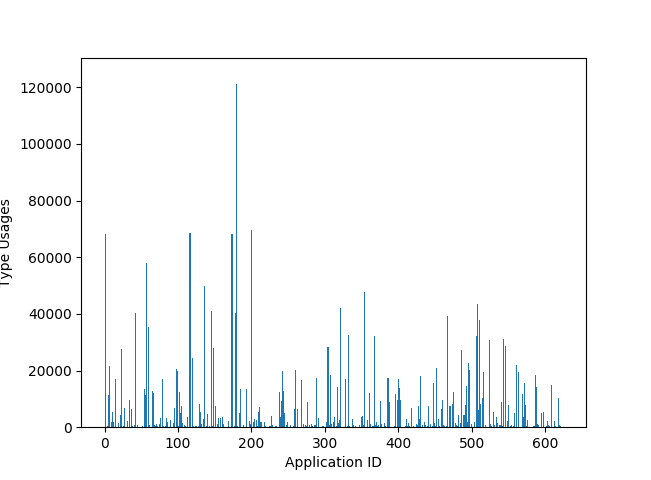
\includegraphics[width=1.1\textwidth]{figures/graph_tus_app}
        \caption{Number of Type Usages per Application}
        \label{fig:tus_app}
    \end{subfigure}
    \begin{subfigure}[h]{0.49\textwidth}
        \centering
        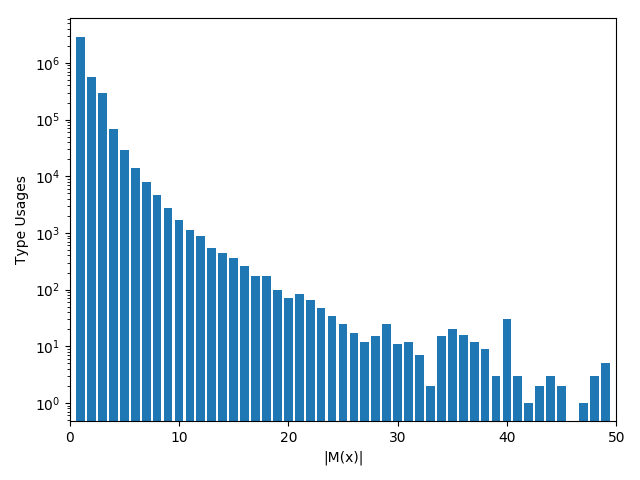
\includegraphics[width=1.1\textwidth]{figures/graph_method_list}
        \caption{Length of Method Lists}
        \label{fig:method_list}
    \end{subfigure}
    \caption{Dataset Overview I}
\end{figure}

%   number of partitions (types + context / types) + maybe verteilung of number of tus per partition (that seems like an interesting / important one!)
In the variation $\text{DMMC}$, a partition is a valid combination of type and context and there are 1,410,709 combinations like that in the dataset.
In the variant $\text{DMMC}_{\text{noContext}}$, the number of partitions is equal to the number of types and the whole dataset includes a total of 202,988 different types.
Since $\text{DMMC}_{\text{class}}$ relies on $A'_\text{noContext}$, the partitions for it are the same as for $\text{DMMC}_{\text{noContext}}$.
However, because we merge the type usages before analyzing them, the total number of type usages for this variant goes down to 958,306.
In Figure \ref{fig:tus_partition}, we have plotted the distribution of type usages per partition for the different variants.
Observer that\ldots 
\todo[inline]{Plot verteilung of TUs per partition!, depending on variant}

\todo[inline]{
    explain why we expect the scores verteilung to be like that
    DEFINITELY somewhere mention the average number of anomalies per app!
        total anomalies: 1650 -> 2.64 avg per app
Does the Strangeness Score behave as expected on Android Apps? (the behavior that I'm expecting is basically a mathematical necessity!)
    do the general assumptions hold? (most tus have a low score, most apps have few findings, etc)
    -> most tus are ``normal'', a few are ``abnormal''
    what do those assumptions mean? -> they expect some kind of uniformity to the type usages, probably mostly present in GUI etc frameworks

mention here: the monperrus2013 p11 highlight? (at least equivalent for my dataset)
    % Second, we note that the distributions of type-usages per type and type-usages per context follow a power-law distribution, which means that a few types and a few contexts trust a large number of type-usages. For instance, for eclipse-swt, the top-20 most popular types (out of 389) cover 62% of the type-usages. This goes along the same line as the results of Baxter et al. [Baxter et al. 2006]
mention somewhere that analysis itself is relatively cheap (especially for new project coming in)
}

% performance: total time +
We perform all our experiments on a MacBook Pro with an Intel\textregistered Core™ i7-3720QM CPU @ 2.60GHz and 16GB of RAM\@.
Extracting the type usages from all applications took a total of 3 hours and 27 minutes, which is an average of around 20 seconds per application.

\begin{figure}[t]
    \centering
    \begin{subfigure}[h]{0.49\textwidth}
        \centering
        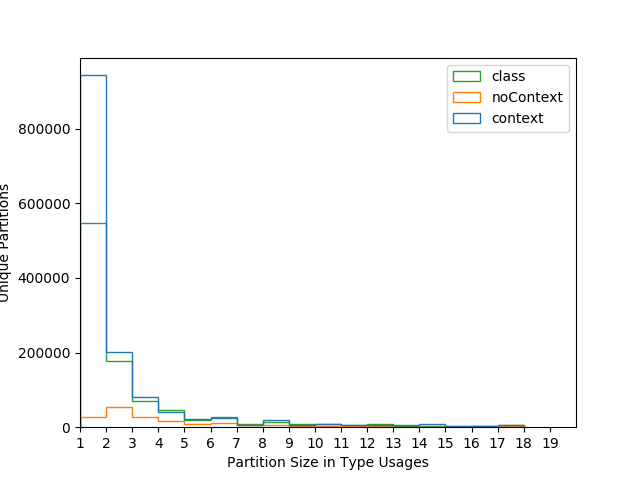
\includegraphics[width=1.1\textwidth]{figures/graph_tus_partition}
        \caption{Distribution of Partition Sizes}
        \label{fig:tus_partition}
    \end{subfigure}
    \begin{subfigure}[h]{0.49\textwidth}
        \centering
        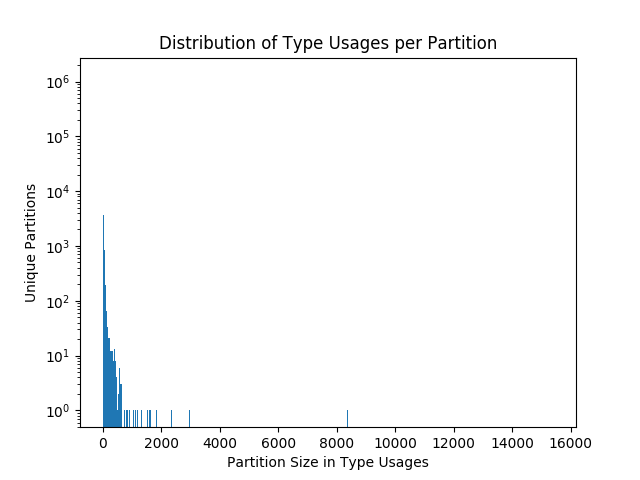
\includegraphics[width=1.1\textwidth]{figures/graph_strangeness}
        \caption{Strangeness Scores using $\text{DMMC}$}
        \label{fig:strangeness}
    \end{subfigure}
    \caption{Dataset Overview II}
\end{figure}

\section{Study Design}
% This section describes how the study, using the information from the study objects, attempts to answer the research questions.

\paragraph{For RQ 1: True vs False Positives}

To determine if an anomaly that was flagged by our implementation is a true finding, we need to manually review it.
Unfortunately, our implementation uncovered too many anomalous type usages to review all of them, prompting us to randomly select 10 applications for detailed analysis.
We examine each anomalous type usages of these applications in detail and classify them as either true or false positive.
This mimics the experience a developer would have when applying our tool to his software.
To answer the research question, we consider the total number of findings per application and the ratio of true to false positive findings.

For RQ 1.2, whether the variations $\text{DMMC}_\text{noContext}$ and $\text{DMMC}_\text{class}$ produce different results, we apply them to the same 10 applications that we sampled for RQ 1.
Once more, we review all findings and classify them as true or false positives.

\paragraph{For RQ 2: Benchmark Results}

% general procedure
To decide if the benchmark results coincide with the results of the manual analysis, we first perform the benchmark itself.
That is, we sample type usages from the dataset, degrade them by removing one of their calls and check if our implementation can detect these known anomalies.
Because we know the correct answer for all degraded type usages, we can use the results to calculate the classical information retrieval metrics:
\begin{description}
    \item [Precision] describes how good our implementation is at suggesting the correct missing call. It is calculated as the weighted confidence the system places on its suggestion.
    \item [Recall] is the percentage of degraded type usages that were detected as anomalous. It tracks if our system correctly detects outliers.
    \item [$\mathbf{F_1}$ score] is the harmonic average of precision and recall.
\end{description}
\todo[inline]{add formeln - right now I'm actually thinking not to
My precision is a different one than the one monp et al use, maybe i should change that? + call it smth different?}

%    pr: sum(confidence(correct prediction) ) / | all queries |
%    rc: sum(correctly detected as anomalie) / | all queries |
%    f1: 2* (pr*rc)/(pr+rc)


% how we want to evaluate the simulation itself
These metrics are already mildly interesting by themselves if we compare them across the three variants $\text{DMMC}$, $\text{DMMC}_\text{noContext}$ and $\text{DMMC}_\text{class}$.
However, as we are not sure about their significance, we also want to evaluate the benchmark itself.
To do so, we compare the benchmark results of each variant to the results of the manual evaluation we performed for RQ 1.
We would expect them to align, that is if one variant produces bad results in the manual evaluation it should also yield bad results in the benchmark.
If there is a serious mismatch between the manual and the benchmark results, this would question the validity of the benchmark.
However, if they agree, it would at least strengthen the idea that the benchmark has some relation to the real world performance of these techniques.

\todo[inline]{
rephrase end of this paragraph - the second part does not actually follow!
am i actually describing ``how to answer the question'' or smth else?
concrete measures for success or not sucess?
}

\paragraph{For RQ 3: Input Size}

Even if we just questioned the validity of the benchmark, we still think that it can offer some insight into the working of our implementation.
Thus, to understand how the quality of findings depends on the amount of input data that is available, we perform a similar kind of benchmark as for RQ 2.
That is, we sample type usages, degrade them by removing a method call and then check if our implementation recognizes them as anomalies.
We calculate the same metrics as in the previous experiment, but this time we consider one additional factor: the size of the partition.
We aim to understand if the partition size has any influence on the quality of results and if so, what partition sizes are advantageous.
In the discussion, we also present some mathematical considerations to support the results.
\todo[inline]{need to explain the partition size at least a little bit, at least reference previous section?
formalize a bit more? aka say if detection rate does this and that?
have the last sentence or not?}
    
\paragraph{For RQ 4: Robustness}

%threefold: mathematical considerations in discussion, benchmark, true BUG + take away
It is difficult to give an accurate answer to the question how sensitive the majority rule is to low-quality input data.
To narrow it down, we perform another simulation experiment, similarly to the one we do for the previous question.
During the experiment, we again sample a type usage from the dataset and degrade it to create a known missing method call.
However, this time, degrading only one type usage is not enough.
Instead, we pick a second random type usage from the same partition as the first one and also remove one of its methods calls, before checking if our implementation can detect the known missing call.
Thus, we simulate the situation that the type in question is in some way difficult to use and it has been used wrongly in multiple places.
We can then calculate precision and recall as before and investigate how this lower quality input data affects the performance of our implementation.
To get the full picture, we observe how the metrics change when we degrade more and more type usages at once.

\todo[inline]{ more formal about performance?
last sentence remix?}

\paragraph{For RQ 5: Other Anomalies}

To understand if the majority rule can also be used to detect superfluous or wrong method calls, we apply our implementation of $\text{DMMC}_\text{superfluous}$ and $\text{DMMC}_\text{wrong}$ to the 10 random applications we sampled for RQ 1.
We manually review their findings in the same manner as we review those of the original variant and label them as true or false positives.

\section{Study Procedure}
% This section describes the nitty gritty details required to implement the study design in reality.
% In principle, they could also be included directly in the description of the study design.
% However, it is easier for the reader to first understand the general idea, and then the details.

The only parameter that our implementation requires is the limit that defines when a type usage is an anomaly.
For this evaluation, we consider type usages with an $\operatorname{S-score}$ bigger than $0.9$ to be anomalies.
This is the value that Monperrus et al.\ suggest and since it implies that 90\% of similar type usages are almost similar it seems like a reasonable cutoff.

\subsection{Manual Review}

% concrete rnd nr gen + results? (already mention the apps -> reference the first rsult figure!)
We used a random number generator\footnote{Google frontpage on: \url{https://www.google.com/search?q=random+number}} to sample the 10 applications that should be examined in detail.
The names of the selected applications can be found in Figure~\ref{fig:manual}.
% manual eval steps?
We analyze all of their type usages with the three different variants $\text{DMMC}$, $\text{DMMC}_{\text{noContext}}$ and $\text{DMMC}_{\text{class}}$ and determine their respective $\operatorname{S-score}$s.
We then manually review all anomalous type usages and carefully consider the source code and the Android API documentation before classifying them as one of the following:
\begin{description}
    \item [real bug (B)] a real defect, change definitely necessary
    \item [real smell (S)] another way of doing things would be better, but probably not a defect in the given instance
    \item [hint (H)] the code is fine, but the pattern is also legitimate; some connection between the methods
    \item [false positive (FP)] the usage is totally fine; no causal relation implying the ``missing'' method must be called
\end{description}

\todo[inline]{ descriptions fine like this? }

We consider bugs and smells to be true positives.
Depending on the quality of results one expects, hints could either be counted towards smells or towards false positives.
\todo{``results one expects'' not clear}
We classify type usages as hints when it makes sense that the pattern exists, because many people will use the methods together and there is some causal connection, but, strictly speaking, there is nothing wrong with the code in question.
As an example, consider the situation in which a developer calls \code{next} on an iterator that he just obtained from a list of size one.
Here, he knows that the iterator contains one element so he does not need to check for it with \code{hasNext}, nonetheless, it is useful to detect locations where \code{next} is invoked without a preceding \code{hasNext}.

\todo[inline]{
a bit more explanation?
    proper example code for better understanding?
    just use the easiest example? -> height and width pairs

additional examples:
only height() or width()
setTitle not called -> not strictly necessary but ``makes sense''
}

\subsection{Automated Benchmark}

% actual setup + degradation mechanism
We perform the benchmark using a custom benchmarking infrastructure written in Python.
It randomly chooses type usages from the dataset and applies a degradation mechanisms to it.
The normal degradation mechanism removes each method call of the selected type usage once and checks for each new version if our implementation of the $\text{DMMC}$ system detects the known anomaly.
To retain a reasonable performance and execution time, we only apply this procedure to a portion of the entire dataset (around 10\%) and then calculate precision and recall as described above.

For the evaluation of RQ 4, we also support a different process of degradation.
Instead of just removing one method call from one type usage, we randomly sample additional type usages from the same partition as the first one and remove one of their calls as well.
\todo[inline]{seems a bit repetitive to the description above, maybe move most stuff here?}

\section{Results \& Interpretation}
% describe results + interpret them with respect to rqs
% A common mistake is to mix the results with the discussion. This makes it harder for the reader to separate backed-up results from speculation.

In the following, we present our results relating to each of the research questions.

\paragraph{For RQ 1: Manual Review}

% concrete techniques and results
\begin{table}[t]
    \centering
    \resizebox{\columnwidth}{!}{%
\begin{tabular}[h]{c|l|r|c|c|c|c|c}
\toprule
Nr & Name & Type Usages & Findings & B & S & H & FP \\
\midrule
1 & ar.rulosoft.mimanganu\_78.apk 			& 11241  & 12 & 1 & 1 & 4 & 6   \\
2 & com.zeapo.pwdstore\_94.apk 				& 12659  & 1  &\cc&\cc& 1 & \cc \\
3 & net.bitplane.android.microphone\_7.apk 	& 80     & \cc&\cc&\cc&\cc& \cc \\
4 & com.quaap.dodatheexploda\_2.apk			& 87     & \cc&\cc&\cc&\cc& \cc \\
5 & com.health.openscale\_23.apk 		   	& 3645   &  3 &\cc& 1 & 2 & \cc \\
6 & se.tube42.kidsmem.android\_16.apk 		& 13547  &  1 &\cc&\cc&\cc&  1 \\
7 & org.billthefarmer.diary\_125.apk	   	& 880    & \cc&\cc&\cc&\cc& \cc \\
8 & org.ligi.blexplorer\_12.apk 	    	& 8350   & \cc&\cc&\cc&\cc& \cc \\
9 & org.kaqui\_27.apk				    	& 1675   & \cc&\cc&\cc&\cc& \cc \\
10 & com.afollestad.nocknock\_13.apk     	& 9547   & \cc&\cc&\cc&\cc& \cc \\
\bottomrule
\end{tabular}}
    \caption{The results of the manual evaluation}\label{fig:manual}
\end{table}

In Table~\ref{fig:manual}, we summarize the results of manually reviewing the findings of the $\text{DMMC}$ variation.
In the entire dataset, on average there are $2.64$ anomalous type usages per application, in our sample there are $1.7$ findings per application.
Of the total 17 findings, 3 are true positives (bug or smell) meaning that $17.65\%$ of findings are true findings.
If we also consider hints to be true findings, this number increases to $58.82\%$.
\todo[inline]{
    order of description makes sense like this or not really?
    do i really want to consider hints as tps?
}

Most of the applications do not exhibit any anomalous type usages and those that do only have a few.
There does not seem to be a relationship between the number of type usages and the number of findings per application.
One of the application is responsible for the majority of findings and also for the majority of false positives.
However, it is also the only one in which a finding indicates a true bug.
In fact, we reported this bug and the maintainer already confirmed and fixed it\footnote{\url{https://github.com/raulhaag/MiMangaNu/issues/535}}.

\begin{table}[t]
    \centering
    \resizebox{\columnwidth}{!}{%
\begin{tabular}[h]{r|r|c|c|c|c|c|c|c|c|c|c|c}
\toprule
%\cmidrule(l){3-10}
    & \multicolumn{6}{c|}{$\text{DMMC}_\text{noContext}$} & \multicolumn{6}{c}{$\text{DMMC}_\text{class}$} \\
App & Type Usages & Findings & B & S  & H    & FP & Type Usages & Findings & B & S & H & FP \\
\midrule
1 & 11241  & 41 (24) & 1 (1)  & 1 (1) & 20 (15) & 19 (7) & 4602 & 28 (14)&1 (1)&  \cc &8 (5)& 19 (8) \\
2 & 12659  & 16 (3)  &  \cc   &  \cc  &  \cc    & 16 (3) & 1560 & 10 (8) & \cc &  \cc &1 (1)&  9 (7) \\
3 & 80     &  0 (0)  &  \cc   &  \cc  &  \cc    &  \cc   & 57   &  0 (0) & \cc &  \cc & \cc & \cc \\
4 & 87     &  0 (0)  &  \cc   &  \cc  &  \cc    &  \cc   & 74   &  0 (0) & \cc &  \cc & \cc & \cc \\
5 & 3645   &  8 (6)  &  \cc   &  \cc  &  3 (1)  &  5 (5) & 1918 &  7 (2) & \cc &  \cc & \cc &  7 (2) \\
6 & 13547  & 23 (0)  &  \cc   &  \cc  &  7 (0)  & 16 (0) & 299  &  0 (0) & \cc &  \cc & \cc & \cc \\
7 & 880    & 21 (2)  &  \cc   &  \cc  &  \cc    & 21 (2) & 427  & 21 (2) & \cc &  \cc & \cc &  21 (2) \\
8 & 8350   &  4 (4)  &  \cc   &  \cc  &  \cc    &  4 (4) & 730  &  2 (2) & \cc &  \cc &1 (1)&   1 (1) \\
9 & 1675   &  2 (1)  &  \cc   &  \cc  &  2 (1)  &  \cc   & 863  &  1 (1) & \cc &  \cc &1 (1)& \cc \\
10& 9547   & 15 (9)  &  \cc   &  \cc  &  \cc    & 15 (9) & 3876 &  4 (3) & \cc &  \cc & \cc &   4 (3) \\
\bottomrule
    \end{tabular}}
    \caption{Comparing $\text{DMMC}_\text{noContext}$ and $\text{DMMC}_\text{class}$. The numbers in brackets indicate findings on the project itself.}\label{fig:manual2}
\end{table}
\todo[inline]{ consider if there is some better way than the brackets? (tried the / but looks like a fraction\ldots) }

In Table~\ref{fig:manual2}, we present the results of applying $\text{DMMC}_\text{noContext}$ and $\text{DMMC}_\text{class}$ to the same applications.
When ignoring the context, the total number of findings grows to 130 of which only 2 are true positive ($1.54\%$), if we also consider the 32 hints to be true positives, the ratio goes up to $26.15\%$.
Since this are a lot of anomalies, we apply a filter to the results that removes any anomaly that does not originate from a class that belongs to the application itself.
As a developer these are the most interesting anomalies, because they can be fixed immediately.
Other anomalies that originate in libraries or other external code will be much harder to fix as they are usually maintained by different people.
The number of findings that remain after applying this filter are displayed in brackets.
It reduces the total number of findings to 49 of which 2 ($4.08\%$) or 19 ($38.78\%$) are true positives depending if we allow hints or not.

The class merge variation detects a total of 73 anomalies with 1 true positive among them ($1.37\%$).
If we factor in the hints, $16.44\%$ of findings are true positives.
By excluding the type usages that do not originate form the application itself, we reduce the total number of anomalies to 32 of which $28.12\%$ are true positives (including hints).
And to clarify, the bug that all of the variations uncover is always the same.

\paragraph{For RQ 2 and 3: Benchmark}

First, we present the benchmark results of the different variants $\text{DMMC}$, $\text{DMMC}_\text{noContext}$ and $\text{DMMC}_\text{class}$ in Table~\ref{fig:bench}.
The original variation has the best precision, but its recall is a little bit worse than that of $\text{DMMC}_\text{noContext}$.
Nonetheless, it narrowly reaches a better $F_1$ score.
The class merge variation exhibits by far the worst results.

We have plotted the development of precision and recall in dependency of the partition size in Figure \ref{fig:partition}.
Especially small partitions (<10 type usages) have very bad recall, we explain the reason for this in the discussion.
Because of this, we have also calculated the performance of our implementation for partitions that contain at least 10 type usage, they are indicated on the right side of Table \ref{fig:bench}.
For these partitions, the superiority of $\text{DMMC}$ over the two other variations is even more clear.
\todo[inline]{ here graph + description of dmmc behavior (all?) over different partition sizes -> make sure the text still fits!}

\begin{table}[ht]
    \centering
    \begin{tabular}[h]{l|c|c|c|c|c|c}
\toprule
 & \multicolumn{3}{c|}{All Partitions}      & \multicolumn{3}{c}{Partitions $> 9$} \\
                                 & Precision & Recall  & $F_1$   & Precision & Recall  & $F_1$ \\
\midrule
$\text{DMMC}$                    & 88.96\%   & 43.52\% & 58.45\% & 90.12\%   & 80.5\%  & 85.04\% \\
$\text{DMMC}_\text{noContext}$   & 59.22\%   & 57.55\% & 58.37\% & 60.06\%   & 64.03\% & 61.98\% \\
$\text{DMMC}_\text{class}$       & 38.89\%   & 24.18\% & 29.82\% & 47.27\%   & 40.05\% & 43.36\% \\
\bottomrule
    \end{tabular}
    \caption{Benchmark Results}\label{fig:bench}
\end{table}

\paragraph{For RQ 4: Robustness}

In Figure \ref{fig:robustness}, we have plotted the evolution of precision and recall as we degrade more and more type usages.
It is obvious that\ldots
\todo[inline]{ benchmark results for degrading 1 or more ADDITIONAL TUS?!  }

\begin{figure}[t]
    \centering
    \begin{subfigure}[h]{0.49\textwidth}
        \centering
        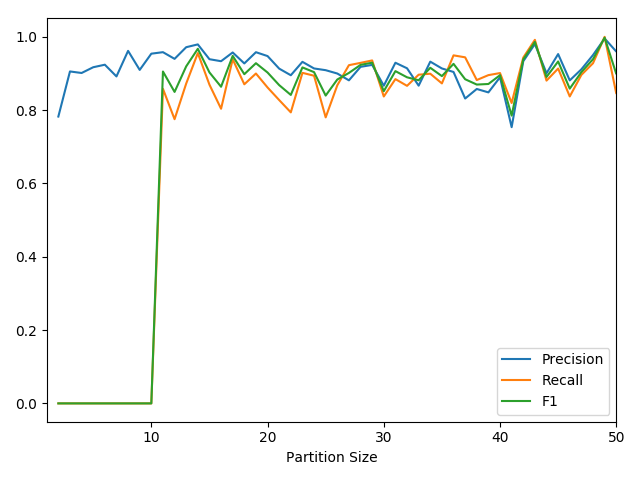
\includegraphics[width=1.1\textwidth]{figures/graph_partition}
        \caption{Metrics depending on Partition Size}
        \label{fig:partition}
    \end{subfigure}
    \begin{subfigure}[h]{0.49\textwidth}
        \centering
        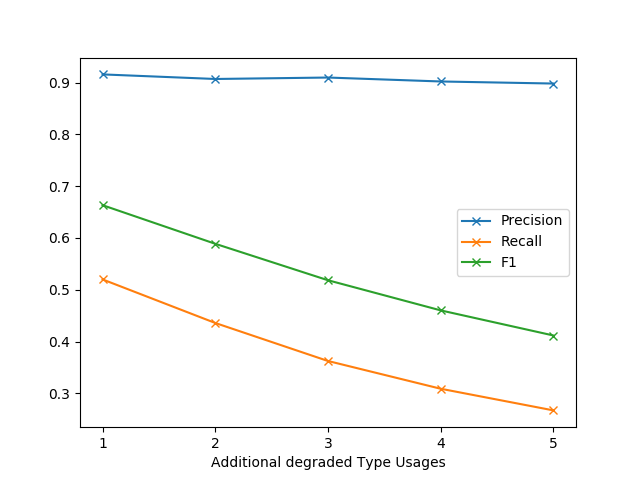
\includegraphics[width=1.1\textwidth]{figures/graph_robustness}
        \caption{Impact of degrading additional Type Usages}
        \label{fig:robustness}
    \end{subfigure}
    \caption{Benchmark Results for RQ 2 and 3}
\end{figure}

\paragraph{For RQ 5: Other Anomalies}

\begin{table}[t]
    \centering
    \begin{tabular}[h]{r|l|r|c|c|c|c|c}
\toprule
& & \multicolumn{2}{c|}{$\text{DMMC}_\text{superfluous}$} & \multicolumn{3}{c}{$\text{DMMC}_\text{wrong}$} \\
Nr & Type Usages & Findings & On Project & Findings & >1 Call & On Project \\
\midrule
 1 &  11241  & 51 & 43 & 95 & 18 & 16  \\
 2 &  12659  & 22 & 19 & 46 &  5 &  5  \\
 3 &  80     &  1 &  1 &  1 & \cc& \cc \\
 4 &  87     &  6 &  6 &  8 &  2 &  2  \\
 5 &  3645   & 22 & 20 & 33 &  9 &  9  \\
 6 &  13547  &  8 &  1 &  1 & \cc& \cc \\
 7 &  880    &  4 &  4 &  2 & \cc& \cc \\
 8 &  8350   &  5 &  2 &  2 & \cc& \cc \\
 9 &  1675   &  4 &  4 &  5 &  1 &  1  \\
10 &  9547   & 26 & 11 & 39 &  9 &  9  \\
\bottomrule
    \end{tabular}
    \caption{Anomalies flagged by $\text{DMMC}_\text{superfluous}$ and $\text{DMMC}_\text{wrong}$}\label{fig:other}
\end{table}

The results of applying the two variations $\text{DMMC}_\text{superfluous}$ and $\text{DMMC}_\text{wrong}$ to the randomly selected applications are depicted in Table \ref{fig:other}.
Both methods detect a lot of anomalies.
During the manual review we did not find a single true positive among them or even a smell or hint, that is, all of these anomalies are false positives.
We again filtered the findings to only include those type usages that originate from the application and not from libraries, however this only reduces the number of findings a little bit.
Before filtering, $\text{DMMC}_\text{superfluous}$ flags a total of 149 type usages as outliers and after 111 remain.

The high number of findings of $\text{DMMC}_\text{wrong}$ is due to a general flaw with the definition of $A'_\text{wrong}$, which we only realized during the evaluation.
The problem is that all type usages that have the same type and make just one call are considered almost equal to each other.
Since the majority rule considers type usages with many almost equal instances to be outliers, this causes the strangeness score of type usages with only one call to be extremely high.
All in all, there is a lot of noise in the data (even if we take the context into account) and the results are nearly meaningless.
Thus, we filter all type usages with only one call from the anomaly list, which reduces them considerably.
However, even the filtered anomalies contain only false positives.

\section{Discussion}\label{sc:disc}
% Interpretation of the results that go further than the research questions. This can, e.g., contain implications for software development.

\paragraph{For RQ 1: True vs False Positives}
% how is the quality of findings (RQ1), how many findings are there, how much work is it to evaluate them

% general
The results of the manual review show that some of the anomalous type usages indeed indicate true bugs or smells.
The number of anomalies per app is relatively small, such that a developer could easily evaluate them himself.
While the manual review was time-consuming, this is partially because we do not know the applications, a developer that is familiar with it would be much faster.
Because of the small sample size, we consider the actual percentages of true positives to be of little import.
\todo[inline]{somehwere here say something about general applicability of this method or only in conclusion?
do i want to explain the one true bug in some more detail or is it fine without?}

% mention side study of top 50 anomalies!
Besides manually reviewing the anomalies in 10 random applications, we also performed a side study on the top 50 anomalies of all applications.
Over its course we did not uncover any additional bugs, but instead a lot of false positives.
Most of these false positives arise out of a small number of failure modes such as:
\begin{itemize}
    \item suggesting a missing call to \code{<init>} (basically never valid, usually the object is a parameter or created by a static function)
    \item not following static functions (in which the suggested missing method is called)
    \item detecting not existing patterns with \code{StringBuilder}
    \item problems with method chaining (does not consider the returned object to be the same as before)
\end{itemize}
Some of these could be fixed rather easily, e.g., we could filter all type usages related to \code{StringBuilder} or anomalies that suggest that a call to \code{<init>} is missing.
Such filters would reduce the number of false positives, but they are also slightly antithetical to the initial idea of avoiding hand crafted rules.
Other problems are more difficult to remedy.
Correctly detecting method chaining seems hard or will at least have some trade-offs.
It seems possible to consider static function evaluations, but we expect it to be expensive in terms of performance.

% no context / class merge
As for RQ 1.1, regarding the comparison between the different variations, it seems clear that the variants $\text{DMMC}_\text{noContext}$ and $\text{DMMC}_\text{class}$ are inferior to the normal $\text{DMMC}$ system.
Not only do they flag more anomalies, the anomalies that they discover are also less relevant.
They find a lot of anomalies in libraries and external code, but even after filtering these out, $\text{DMMC}$ is still better.
\todo{fyi the filter only removes 2 FP anomalies form the normal variation}

\todo[inline]{ even mention this? I think not right now\ldots

failure modes: wihtout context: anomalies when clases call functions in itself
many repetitions of identical findings
Kotlin thingy (even mention SC thing?)
-> not many kotlin apps -> easy to be an outlier for some stuff (init for example), etc
failure mode: kotlin -> outlier generally
}

\paragraph{For RQ 2: Benchmark Results}

For this question, we compare the results of the benchmark with those of the manual evaluation.
In the manual review $\text{DMMC}$ is the superior method by far.
From the benchmark results this is not as clear, it has the best precision but the recall is worse than that of $\text{DMMC}_\text{noContext}$.
If we consider the benchmark results for partitions that have at least 10 type usages, $\text{DMMC}$ becomes the sole leader.
This is due to the fact that $\text{DMMC}_\text{noContext}$ does not have many partitions that are smaller than 10 and, as we will explain in the next paragraph, 10 is the crucial minimal size for this method to detect anything.
Thus, it seems fair to conclude that the results of the manual evaluation align with the benchmark results.
This is not enough to conclude that the benchmark itself is a good or realistic measure for the performance of different missing method call detectors.
\todo{-> critical assumption not further looked at (they are the same as real mmc bugs)}
However, at least our results at least do not indicate the opposite: that the benchmark is a bad measure of their performance.
\todo[inline]{not super happy with the end\ldots}

\paragraph{For RQ 3: Input Size}

The graph in Figure \ref{fig:partition} shows clearly that the systems accuracy increases with the size of the partition.
Especially for partitions smaller than 10, the recall is terrible.
To explain this, consider the strangeness score of a true bug $b$.
If there are no instances equal to $b$, then $|E(b)|=1$ and $\operatorname{S-score}(b)=1-\frac{1}{1+|A(b)|}$.
We consider type usages with a strangeness score of more than $0.9$ to be anomalies, so $b$ can only be flagged as anomalous as soon as there are at least $9$ instances that are almost similar to it.
It follows that there must be at least 10 type usages within the same partition to have even a theoretical chance of detecting any outliers.

Now consider that the $\text{DMMC}$ variant that takes the context into account has shown the best performance and the distribution of partitions presented in Figure \ref{fig:tus_partition}.
Even in our large dataset of 625 applications, most partitions are still rather small.
In fact, a majority of type usages belong to partitions that are smaller than the necessary minimum of 10, meaning that our system can not actually detect any bugs or other outliers among them.
\todo{is this true + what are exact numbers?}
All in all, it seems that it is difficult to obtain the necessary rich dataset, even when taking a lot of code into consideration.

\todo[inline]{more clearly work towards conclusion: it is difficult to get the right kind of data!

mention ts? (I'm slightly against it)
We also applied our implementation to a medium sized industry application (TS!) (mention LOC) and the results it produced supported this intuition, being of rather poor quality.
any other actual results on this? I don't actually think so\ldots }

\paragraph{For RQ 4: Robustness}

The graph in Figure \ref{fig:robustness}  makes it plain that the accuracy of our implementation decreases tremendously when we introduce additional degraded type usages into the data.
% then math considerations
Since we are not confident in the applicability of the benchmark, we also make a mathematical consideration with regards to the behavior of the $\operatorname{S-score}$.
In the previous paragraph, we already considered the true bug $b$ with no equal instances.
We need at least 9 almost similar instances to detect it.
Now, consider another true bug $b'$ that has one exactly similar neighbor, that is $|E(b')|=2$ and thus $\operatorname{S-score}(b')=1-\frac{2}{2+|A(b)|}$.
In other words, we can only detect these anomalous type usages if there are at least 18 instances that are almost equal to them, double as many as before.

%  verweis auf partitions sizes
The more errors there are in our dataset, the more data we need to detect them.
The impact of this becomes especially clear if one consults the graph in Figure \ref{fig:tus_partition} displaying the distribution of partition sizes in our dataset.
Most of them are small and thus having an additional mistake in the dataset can easily prevent our implementation from flagging both as an anomaly.
% -> tentative answer: it's a little bit sensible to bad inputs
Al in all, we tentatively conclude that the majority rule is relatively sensible to erroneous input data.

\paragraph{For RQ 5: Other Anomalies}

Our implementations of $\text{DMMC}_\text{superfluous}$ and $\text{DMMC}_\text{wrong}$ both detect a relatively high number of findings without any actual success.
More damningly, upon manual review of the findings it becomes clear that the patterns which they extract do not make any sense.
None of the suggested changes, be it removing a method call or exchanging one, did have any causal justification and it seems clear that they are only artefacts of randomness in the data.
\todo{example?, bit better description\ldots}
All in all, we do not consider our naive application of the majority rule useful for detecting superfluous or wrong method calls.

\section{Threats to Validity}
% all threats, i.e. reasons why the study results could be wrong. Ideally, it then treats every single threat and describes what you did to make sure that this threat does not invalidate your study results

There are several internal and external threats to the validity of this study.

% internal: reasons why the results could be invalid for your study objects
As for the internal threats, the strongest one seems to be that our manual evaluation is biased and subjective.
Unfortunately, we do not have the resources to let multiple developers review the anomalies.
To prevent judging the results too harshly, we introduce the hint category which contains many findings that are not bugs or even smells, but rather subtle pointers for something that could cause problems.
If we acknowledge them as true positives, we get a favorable picture of the capabilities of our implementation.
On the other hand, we can also exclude the hints and thus, obtain a lower bound.
The truth probably lies somewhere between them.

The only parameter that our implementation uses is the strangeness value above that a type usages is considered an anomaly.
We could set it lower to improve the recall or higher in an attempt to improve the precision.
We cannot present any hard data on this, but during the manual review, we often observed that even type usages with a strangeness value much higher than $0.9$ were not really true positives.
Because of this, we deem it unlikely that reducing the cutoff to lower value would improve the results.
As for increasing the cutoff, we think that the average number of findings is acceptable and does not need to be lowered.

We already mention the problems of the automatic benchmark in Section \ref{sc:rq}.
It is simply not clear how similar degraded type usages are to missing method calls in the wild.
Thus, to prevent relying too much on the benchmark, we also take some mathematical considerations into account before answering RQ 3 and 4.

% external: reasons why the results encountered for the study objects might not be transferable to other objects.
% In the example, the way we chose the study objects (through our personal network) might bias our results. To mitigate this threat, we at least chose systems that had different characteristics, such as programming language, development contractor and age.
Regarding the external threats, we have to review our study objects.
We use a large dataset and choose the applications for manual review at random, to avoid getting results that rely on outliers.
To hedge against underrating our implementation, we performed a side study on the top 50 anomalies among all applications.
However, of course all study objects are Android applications and open source.
We think that the Android framework should be a favorable for this method because of its focus on user interface, but it is feasible that this method works much better on another OOP language or simply another Java framework.
Finally, it is not clear if open source applications are comparable to commercial software in terms of size or quality.

\todo[inline]{
schönere aufbauen iwie? vllt mit ende starten -> we dont know this, but at least we are selecting at random and there is a wide variety of software in Fdroid oä

open source: potentially quality lower etc, but that should make it EASier to find bugs\ldots}

